Distillation towers are integral units in industrial processes that require the separation of
mixtures of different components into products based on their relative volatility. Heavy oil
upgrading facilities utilize distillation towers to separate feed mixtures into various products based on their specific gravity.  For many chemical plants, the distillation tower can account up to 50\% of the total operating cost, making optimization of the distillation tower a low hanging fruit in terms of cost savings.  

Flooding is a common and costly problem in industrial distillation towers.  Flooding occurs when liquids are entrained in the vapour due to abnormally high vapour flow rates.  Moreover, the excess pressure also causes liquid holdup in the higher plates of the distillation tower. Ultimately, this leads to significant reduction in separation efficiency causing a loss in production, wasted energy, and off-spec products.

In this chapter, a reinforcement learning based fault tolerant controller will be introduced to mitigate damage caused by flooding events in distillation towers.  The process will first be introduced. Then, common faults will be introduced into the system.  Following that, PID, MPC and RL will all be used to try to guide the system out of the fault situation.  Finally, the performance of each controller will be compared.

\section{Process Introduction}
The Wood-Berry distillation tower, located in the University of Alberta, will be used for this study to compare the performance between PID, MPC, and RL controllers in a fault positive scenario.  

\subsection{Process Description}
Distillation is the process of separating a liquid or vapour mixture of two or more components into desirable purities through the addition or removal of heat. The fundamental theory of distillation is that low boiling point components are richer in the vapour of a boiling mixture, while the liquids would contain more of the less volatile components \cite{distillation_intro}.  Liquids exit the bottom of the distillation tower and is sent to a reboiler, where heat is added to vaporize any straggling high volatility product to ensure maximum separation. Similarly, vapour from the top of the tower is sent to a condenser, where heat is removed and additional low volatility components may be recovered. The condensed vapour is collected in the reflux drum, and will be recycled back into the distillation tower. Typically, distillation columns are large vertical drums with evenly spaced trays to enhance separation of the vapour and liquid components \cite{mpc_for_distillation_tower}.  The tower is separated into two sections.  The rectifying section is located between the feed tray and the top of the column and aims to concentrate light components in the vapour phase.  Moreover, the stripping section is located between the feed tray and the column bottom and is used to concentrate the heavier components in the liquid phase \cite{henry_distillation}.

A process flow diagram of the Wood-Berry tower is shown in Figure \ref{fig: woodberry}.  It contains one feed stream and two outlet streams.  Commonly, the feed stream is characterized by the inlet mol composition, $Z_f$.  The top product, also called distillate, is characterized by mass fraction, $X_D$.  The bottom product is characterized by mass fraction, $X_B$.  The process has two control inputs and two outputs. The control inputs of the system are the reflux and steam flow rates, $R$ and $S$.  The outputs are the distillate and bottoms product mass compositions, $X_D$ and $X_B$.

\begin{figure}[h]
    \centering
    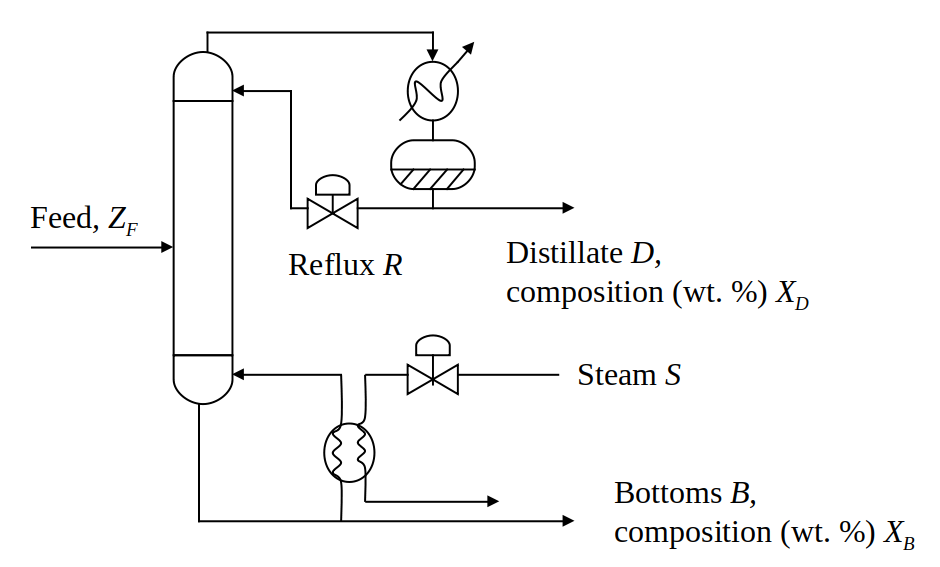
\includegraphics[scale=0.45]{images/woodberry.png}
    \caption{A schematic diagram of a binary distillation tower.  Original figure from Dr. Seborg from UC Santa Barbara with edits for enhanced clarity.}
    \label{fig: woodberry}
\end{figure}

In the Wood-Berry distillation tower, the goal is the complete separation of methanol and water.  Methanol has a boiling point of 64.7 \textdegree C whereas pure liquid water has a boiling point of 100 \textdegree C \cite{sonntag_thermo}. Thus, making methanol the distillate and water is the bottoms product. $X_D$ and $X_B$ are the distillate and bottoms $\%MeOH$, respectively. The two manipulated variables in the system are the reflux flow rate, $R \; (lb/min)$ and the steam flow rate, $S \; (lb/min)$.  The objective of the manipulated variables is to achieve 100\% $X_D$, while maintaining $X_B$ at 0\%. Additional detailed information about the operation and inner workings of distillation towers can be found in \cite{henry_distillation}.  

\subsection{Wood-Berry Models}
The transfer functions that realize  the Wood-Berry distillation tower is given in Equation \ref{eq: woodberry_tf} \cite{mpc_for_distillation_tower}.

\begin{equation}
    \centering
    \begin{bmatrix}
        Y_1(s) \\
        Y_2(s) 
    \end{bmatrix}
    =
    \begin{bmatrix}
        G_{11}  & G_{12} \\
        G_{21}  & G_{22}
    \end{bmatrix}
    \begin{bmatrix}
        u_1(s) \\
        u_2(s)
    \end{bmatrix}
    \label{eq: woodberry_tf}
\end{equation}
where: 
\begin{equation}
    \centering
        {\large
        \begin{matrix}
            G_{11} = \frac{12.8e^{-s}}{16.7s + 1}     &     G_{12} = \frac{-18.9e^{-3s}}{21s + 1} \\
            G_{21} = \frac{6.6e^{-7s}}{10.9s + 1}     &     G_{22} = \frac{-19.4e^{-3s}}{14.4s + 1}
        \end{matrix}}
    \label{eq: transfer_functions_woodberry}
\end{equation}

Due to the difficulty of transfer function simulations in Python, the model was converted into state space form.  After conversion, two control loops had to be developed to realize the system because of inconsistencies in the input time delay.  Equations \ref{eq: x_ss_eq1} and \ref{eq: x_ss_eq2} are the state space models for the distillate and bottoms compositions, respectively.  The initial states were assumed to be all zero.

\begin{equation}
    \centering
    x_0 = 
    \begin{matrix}
        [0 & 0 & 0 & 0]
    \end{matrix}
\end{equation}

\begin{equation}
    \centering
    \begin{bmatrix}
        \dot{x_1} \\
        \dot{x_2} \\
        \dot{x_3} \\
        \dot{x_4} 
    \end{bmatrix}
    =
    \begin{bmatrix}
        -0.0599     &     0     &     0     &     0 \\
        0           &  -0.0917  &     0     &     0 \\
        0           &     0     &   -0.0476 &     0 \\
        0           &     0     &     0     &  -0.0694
    \end{bmatrix}
    \begin{bmatrix}
        x_1 \\
        x_2 \\
        x_3 \\
        x_4 
    \end{bmatrix}
    +
    \begin{bmatrix}
        1     &     0  \\
        1     &     0  \\
        0     &     1  \\
        0     &     1
    \end{bmatrix}
    \begin{bmatrix}
        u_1(t - 1) \\
        u_2(t - 3)
    \end{bmatrix}
    \label{eq: x_ss_eq1}
\end{equation}

\begin{equation}
    \centering
    X_D(t) =  
    \begin{matrix}
        [0.7665 & 0 & -0.9 & 0]
    \end{matrix}
    \begin{matrix}
        [x_1 & x_2 & x_3 & x_4]^T
    \end{matrix}
    \label{eq: X_D_output}
\end{equation}

\begin{equation}
    \centering
    \begin{bmatrix}
        \dot{x_1} \\
        \dot{x_2} \\
        \dot{x_3} \\
        \dot{x_4} 
    \end{bmatrix}
    =
    \begin{bmatrix}
        -0.0599     &     0     &     0     &     0 \\
        0           &  -0.0917  &     0     &     0 \\
        0           &     0     &   -0.0476 &     0 \\
        0           &     0     &     0     &  -0.0694
    \end{bmatrix}
    \begin{bmatrix}
        x_1 \\
        x_2 \\
        x_3 \\
        x_4 
    \end{bmatrix}
    +
    \begin{bmatrix}
        1     &     0  \\
        1     &     0  \\
        0     &     1  \\
        0     &     1
    \end{bmatrix}
    \begin{bmatrix}
        u_1(t - 7) \\
        u_2(t - 3)
    \end{bmatrix}
    \label{eq: x_ss_eq2}
\end{equation}

\begin{equation}
    \centering
    X_B(t) =  
    \begin{matrix}
        [0 & 0.6055 & 0 & -1.3472]
    \end{matrix}
    \begin{matrix}
        [x_1 & x_2 & x_3 & x_4]^T
    \end{matrix}
    \label{eq: X_B_output}
\end{equation}

\subsection{Model Validation}

To ensure the state space model is equivalent to the original transfer function model, step tests were conducted on both systems.  The input for $u_1$ and $u_2$ were set to 1 for 150 time steps and the output trajectory is shown in Figure \ref{fig: step_test_plots} for both the transfer function and state space models. From Figure \ref{fig: step_test_plots}, it can be seen that both trajectories are identical. 

\begin{equation}
    \centering
    u_t = 
    \begin{bmatrix}
        1  &  1  &  ...  &  1 \\
        1  &  1  &  ...  &  1
    \end{bmatrix}_{2 \times N}
    \; where \; N = 150
    \label{eq: step_test_input}
\end{equation}

\begin{figure}[h]
    \centering
    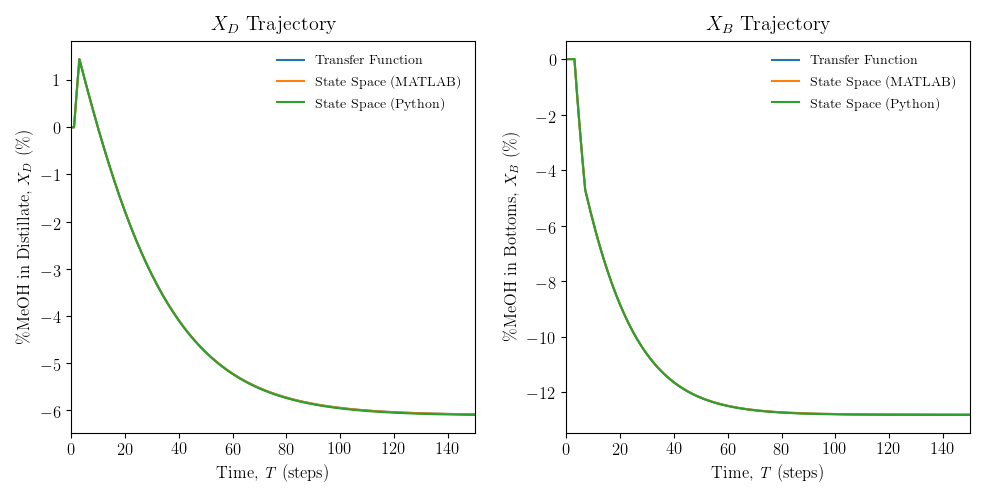
\includegraphics[scale=0.42]{images/step_test_plots.png}
    \caption{A comparison of the $X_D$ and $X_B$ trajectories for the transfer function and state space models}
    \label{fig: step_test_plots}
\end{figure}

To further confirm the validity of the results, the steady state problem was also calculated to ensure simulations were giving correct results. During steady state, the change in states, $\dot{x_i}$, are zero.

\begin{equation}
    \centering
    \dot{x_1}, \dot{x_2}, \dot{x_3}, \dot{x_4} = 0
\end{equation}

Given that $u_1$ and $u_2$ are one (from Equation \ref{eq: step_test_input}), all states can be analytically solved.  Delays will be omitted because the inputs are assumed to be identical for 150 time steps. Equations \ref{eq: x1_analytical} - \ref{eq: x4_analytical} shows the numerical solution to each state at steady state.

{\setstretch{0.5}
\begin{equation}
    \centering
    x_1 = 16.7
    \label{eq: x1_analytical}
\end{equation}

\begin{equation}
    \centering
    x_2 = 10.9
    \label{eq: x2_analytical}
\end{equation}

\begin{equation}
    \centering
    x_3 = 21.0
    \label{eq: x3_analytical}
\end{equation}

\begin{equation}
    \centering
    x_4 = 14.4
    \label{eq: x4_analytical}
\end{equation}
}

Combining Equations \ref{eq: X_D_output} and \ref{eq: X_B_output} with Equations \ref{eq: x1_analytical} - \ref{eq: x4_analytical}, the steady state values for $X_D$ and $X_B$ are given by Equations \ref{eq: final_xd} and \ref{eq: final_xb}, respectively. \\

{\setstretch{0.5}
\begin{equation}
    \centering
    X_D = 0.767x_1 - 0.900x_3
\end{equation}

\begin{equation}
    \centering
    X_D = 0.767(16.7) - 0.900(21.0) = -6.1
    \label{eq: final_xd}
\end{equation}

\begin{equation}
    \centering
    X_B = 0.606x_2 - 1.35x_4
\end{equation}

\begin{equation}
    \centering
    X_B = 0.606(10.9) - 1.35(14.4) = -12.8
    \label{eq: final_xb}
\end{equation}
}

Comparing the analytical steady state solutions found for $X_D$ and $X_B$ to the final steady state values reached in Figures \ref{fig: step_test_plots} it can be seen that the solutions are identical; further confirming the models validity.

\section{Finding the Optimal Solution}

The optimal solution for the Wood-Berry distillation column is given by Equations \ref{eq: xd_optimal} and \ref{eq: xb_optimal}, i.e., perfect separation of methanol from water. To obtain the ideal steady state inputs, $u_1^*$ and $u_2^*$, Equations \ref{eq: final_xd} and \ref{eq: final_xb} are solved with the conditions:

{\setstretch{0.5}
\begin{equation}
    \centering
    X_D^* = 100
    \label{eq: xd_optimal}
\end{equation}

\begin{equation}
    \centering
    X_B^* = 0
    \label{eq: xb_optimal}
\end{equation}
}

By solving Equations \ref{eq: X_D_output} and \ref{eq: X_B_output} for $x_1, x_2, x_3$ and $x_4$ when delays are omitted and $\dot{x}_i$ are zero, the following equations are obtained: \\

{\setstretch{0.5}
\begin{equation}
    \centering
    x_1 = 16.7u_1
    \label{eq: x_1_ss_opt}
\end{equation}

\begin{equation}
    \centering
    x_2 = 10.91u_1
\end{equation}

\begin{equation}
    \centering
    x_3 = 21.0u_2
\end{equation}

\begin{equation}
    \centering
    x_4 = 14.4u_2
    \label{eq: x_4_ss_opt}
\end{equation}
}

Combining Equations \ref{eq: x_1_ss_opt} - \ref{eq: x_4_ss_opt} with \ref{eq: final_xd} and \ref{eq: final_xb}, the optimal inputs are analytically solved and are given by: \\

{\setstretch{0.5}
\centering
$X_D^* = 0.767(16.7)u_1 - 0.900(21.0)u_2$

\begin{equation}
    \centering
    100 = 12.8u_1 - 18.9u_2
    \label{eq: opt_xd}
\end{equation}
}

{\setstretch{0.5}
\centering
$X_B^* = 0.606(10.9)u_1 - 1.347(14.4)u_2$

\begin{equation}
    \centering
    0 = 6.6u_1 - 19.5u_2
    \label{eq: opt_xb}
\end{equation}
}

Combining Equations \ref{eq: opt_xd} and \ref{eq: opt_xb}, the optimal steady state inputs are: \\

{\setstretch{0.5}
\begin{equation}
    \centering
    u_{1, ss}^* = 15.7
\end{equation}

\begin{equation}
    \centering
    u_{2, ss}^* = 5.3
\end{equation}
}

\subsubsection{Simulating the Optimal Solution}
Figures \ref{fig: optimal_ss_xd_xb} show the trajectories of $X_D$ and $X_B$ given the optimal control input.

\begin{figure}[h]
     \centering
      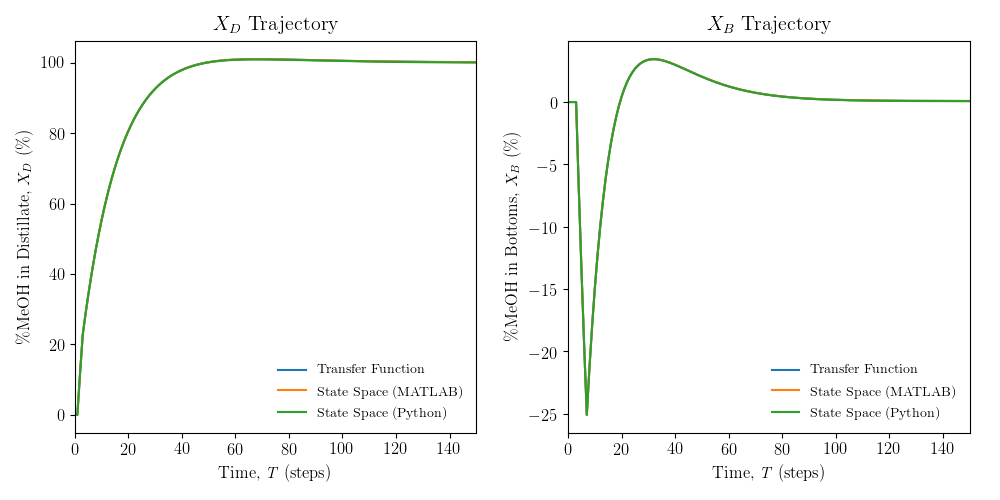
\includegraphics[scale=0.42]{images/optimal_input_plots.png}
     \caption{Trajectories of $X_D$ and $X_B$ using optimal steady state inputs, $u_{ss}^*.$}
     \label{fig: optimal_ss_xd_xb}
\end{figure}

\section{Design of the Control System}
Controllers must first be designed to control the system to desired set-points.  Given that the system has multiple inputs and multiple outputs (MIMO), two different control designs can be explored.  The first control design is building one multi-variate controller capable of controlling both inputs, given feedback from both outputs.  The second design decomposes the system into smaller sub-systems so multiple single-input single-output (SISO) controllers can be applied for control.  In this study, two SISO PID controllers will be designed for regulatory control.  Then, a model predictive controller (MPC) will be designed as a multi-variate supervisory controller.  

\subsection{Relative Gain Array}
Due to the MIMO system being coupled (i.e, the control signal sent to one actuator will indirectly affect the output signal of the second control loop), the relative interactions between the control actions needs to be explored. Exploration of the coupling effect is required to tune the control system appropriately and ensure instabilities do not exist. One simple way to investigate the degree of coupling is to compute the relative gain matrix, $\Lambda$. Using the relative gain matrix, the proper input output pairing can also be determined \cite{RGA}. A flaw in the relative gain array is the lack of consideration for time delays.  However, the PID controllers will be evaluated every 10 seconds, so the effect of delays are assumed to be negligible.  To solve for the relative gains, the process gain, $K_{process}$, for each transfer function in the system must first be identified.  The definition of $K_{process}$ is given in Equation \ref{eq: process_gain}:

\begin{equation}
    \centering
    K_{process} = \frac{\partial y_i}{\partial u_i} \approx \frac{\varDelta y_i}{\varDelta u_i}
    \label{eq: process_gain}
\end{equation}
where $\partial y_i$ and $\partial u_i$ are the partial derivative of the outputs and inputs, respectively. The function can be approximated by the change in $y_i$ and $u_i$, given the step sizes are sufficiently small.  Intuitively, $K_{process}$ describes the relative effect of $u_i$ on $y_i$.  

The standard form of a transfer function is given by:

\begin{equation}
    \centering
    G(s) = \frac{Y(s)}{U(s)} = \frac{K}{\tau s + 1}
\end{equation}
where $K$ and $\tau$ are the process gain and time constant, respectively.

Referring to Equation \ref{eq: transfer_functions_woodberry}, all the transfer functions are in standard form.  Therefore, their process gains are simply the coefficient of the numerators and are:

\begin{equation}
    \centering
    K_{ij} =
    \begin{bmatrix}
    12.8     &     -18.9 \\
    6.6      &     -19.4 
    \end{bmatrix}
    \label{eq: process_gains}
\end{equation}
where $i$ denotes the $i^{th}$ element in each row and $j$ denotes the $j^{th}$ element in each column (e.g. $K_{18}$ denotes the element in the first row and 8th column).

The general form of the system outputs is:

\begin{equation}
    \centering
    \begin{bmatrix}
        y_1 \\
        y_2
    \end{bmatrix}
    =
    \begin{bmatrix}
        K_{11}  &  K_{12} \\
        K_{21}  &  K_{22}
    \end{bmatrix}
    \begin{bmatrix}
        u_1 \\
        u_2
    \end{bmatrix}
    \label{eq: general_ss_form}
\end{equation}
where $y_1$ and $y_2$ are the system outputs.  Subsequently, $u_1$ and $u_2$ are the system inputs. \\

\noindent
The standard form of Equation \ref{eq: general_ss_form} is:
{\setstretch{0.5}
\begin{equation}
    \centering
    y_1 = K_{11}u_1 + K_{12}u_2
    \label{eq: y1_iol}
\end{equation}
\begin{equation}
    \centering
    y_2 = K_{21}u_1 + K_{22}u_2
    \label{eq: y2_iol}
\end{equation}}

\noindent
The relative gain between $y_i$ and $u_j$, $\lambda_{ij}$, is given by:

\begin{equation}
    \centering
    {\Large
    \lambda_{ij} = \frac{(\frac{\partial y_i}{\partial u_j})|_{U}}{(\frac{\partial y_i}{\partial u_j})|_{Y}}
    }
    \label{eq: relative_gain}
\end{equation}
where $U = \mathcal{U}, U \neq u_j$ and $Y = \mathcal{Y},Y \neq y_i$.  The numerator and denominator of the relative gain represents the open loop and closed loop gain between $y_i$ and $u_j$, respectively.

\noindent
Solving for the numerator of $\lambda_{11}$ yields:
\begin{equation}
    \centering
    \left.\frac{\partial y_1}{\partial u_1} \right \vert_{u_2} = \frac{\partial}{\partial u_1}[K_{11}u_1 + K_{12}u_2] = K_{11}
\end{equation}

\noindent
Similarly, solving for the denominator of Equation \ref{eq: relative_gain} gives:
\begin{equation}
    \centering
    \left.\frac{\partial y_1}{\partial u_1}\right\vert_{y_2} = \frac{\partial}{\partial u_1}[K_{11}u_1 + K_{12}u_2]
    \label{eq: y2_relative_gain}
\end{equation}
Since $y_2$ does not appear in Equation \ref{eq: y1_iol}, Equation \ref{eq: y2_iol} must be substituted into Equation \ref{eq: y1_iol}.  Because $y_2$ is a deviation variable, $y_2 = 0$ giving:

\begin{equation}
    \centering
    0 = K_{21}u_1 + K_{22}u_2
    \label{eq: u2_relative_gain1}
\end{equation}
solving for $u_2$:
\begin{equation}
    \centering
    u_2 = \frac{-K_{21}u_1}{K_{22}}
    \label{eq: u2_relative_gain2}
\end{equation}

\noindent
Substituting Equation \ref{eq: u2_relative_gain2} into Equation \ref{eq: y2_relative_gain} and solving the partial derivative yields:

\begin{equation}
    \centering
        (\frac{\partial y_1}{\partial u_1})_{y_2} = \frac{\partial}{\partial u_1}[K_{11}u_1 - \frac{K_{12}K_{21}u_1}{K_{22}}] = K_{11} - \frac{K_{12}K_{21}}{K_{22}}
\end{equation}
The relative gain array, $\Lambda$, is:

\begin{equation}
    \centering
    \Lambda = 
    \begin{bmatrix}
    \lambda_{11}   &   \lambda_{12}   \\
    \lambda_{21}   &   \lambda_{22}
    \end{bmatrix}
\end{equation}
and satisfies the following conditions given $\Lambda$ is a square matrix:
{\setstretch{0.5}
\begin{equation}
    \centering
    \sum_{j = 1}^N \lambda_{ij} = 1
\end{equation}
\begin{equation}
    \centering
    \sum_{i = 1}^M \lambda_{ij} = 1
\end{equation}
\begin{equation}
    \centering
    \lambda_{ij} = \lambda_{ji}
\end{equation}}
where N and M are the number of elements in the rows and columns, respectively.

\noindent
Using the above conditions, the relative gain matrix can be simplified to:
\begin{equation}
    \centering
    \begin{bmatrix}
     K_{11} - \frac{K_{12}K_{21}}{K_{22}}   &   1 - K_{11} - \frac{K_{12}K_{21}}{K_{22}}   \\
     1 - K_{11} - \frac{K_{12}K_{21}}{K_{22}}   &   K_{11} - \frac{K_{12}K_{21}}{K_{22}}
    \end{bmatrix}
    \label{eq: final_relative_gain_array}
\end{equation}
Substituting values from Equation \ref{eq: process_gains} into Equation \ref{eq: final_relative_gain_array} results in:
\begin{equation}
    \centering
    \Lambda = 
    \begin{bmatrix}
     2   &   -1   \\
     -1  &    2
    \end{bmatrix}
    \label{eq: relative_gain_array_w_values}
\end{equation}

The physical meaning of the relative gains are summarized in Table \ref{tab: relative_gains} \cite{process_control_design_sim}.
\begin{table}[h]
    \centering
    {\setstretch{1.5}
    \begin{tabular}{ c | p{12cm} }
        Magnitude of $\lambda_{ij}$  & Physical Meaning \\
        \hline
        $\lambda_{ij} = 1$ & Open and closed loop gains are identical; no interaction effects for pairing $y_i$ and $u_j$ \\
        $\lambda_{ij} = 0$ & Open loop gain is zero; $u_j$ has no effect on $y_i$ \\
        $ 0 < \lambda_{ij} < 1$ & Closed loop interactions increases gain \\
        $\lambda_{ij} > 1$ &  Closed loop interactions reduce gain \\
        $\lambda_{ij} < 0$ & Open and closed loop gains have opposing effects \\
    \end{tabular}}
    \caption{Description of relative gain values.}
    \label{tab: relative_gains}
\end{table}

From $\Lambda$, $\lambda_{12}$ is negative, meaning that pairing $y_1$ with $u_2$ results in opposing open and closed loop gains.  A similar outcome can be seen by pairing $y_2$ with $u_1$.  Both scenarios should be avoided to ensure stability in the system. From Table \ref{tab: relative_gains}, $\lambda_{11}, \lambda_{22} = 2$.  Although this is better than the relative gain being negative, it is still far from 1, so a decoupler should be implemented to achieve independent control of $y_1$ and $y_2$ using $u_1$ and $u_2$.

\subsection{Simple Decoupling using Equivalent Transfer Functions}
In literature, there are three popular decoupling methods: i) ideal, ii) simplified, and iii) inverted [Cite].  The ideal decoupling method requires inversing of the transfer functions, and leads to modelling errors [Cite].  The simplified method overcomes these shortcomings, however, the decoupled process cannot be directly used for controller design without the model reduction technique [Cite].  The inverted method combines all the advantages of the ideal and simplified methods, but high dimensional systems may be physically unrealizable, and it is also more prone to errors [cite].  Rajapandiyan et al. (2012) proposed a new method to perform decoupling of systems with time delays that improve upon the classical methods.  

First, the multi-loop system is decoupled into multiple single loop systems using the simplified decoupler matrix.  The decoupled process is then approximated using its effective open-loop transfer function (EOTF).  Subsequently, Rajapandiyan et al. (2012) showed that the EOTF was exactly equivalent to the equivalent transfer function (ETF) when the system is open-loop stable and there are no oscillatory characteristics.  From the EOTFs, the decentralized PID controllers can then be designed using the simplified internal model control (SIMC) method. 

Referring to Equation \ref{eq: woodberry_tf}, it can be seen that the Wood-Berry distillation system is open-loop stable because all poles are in the left-half plane.  From Figure \ref{fig: step_test_plots}, the system also has no oscillations during step tests. Thus, the system in this study satisfies the requirements posed by Rajapandiyan et al. (2012). 

\subsubsection{Decoupler Design}
Figure \ref{fig: control_loop_IOL} shows the simplified closed-loop control system for the Wood-Berry distillation tower \cite{decoupler_design}.  $G_c(s)$ and $G(s)$ are the distributed controller matrix and the process transfer functions, respectively, and are shown in Equations \ref{eq: transfer_functions_woodberry} and \ref{eq: controller_tf_iol}.  $y_{r_1}$ and ...

\begin{figure}
    \centering
    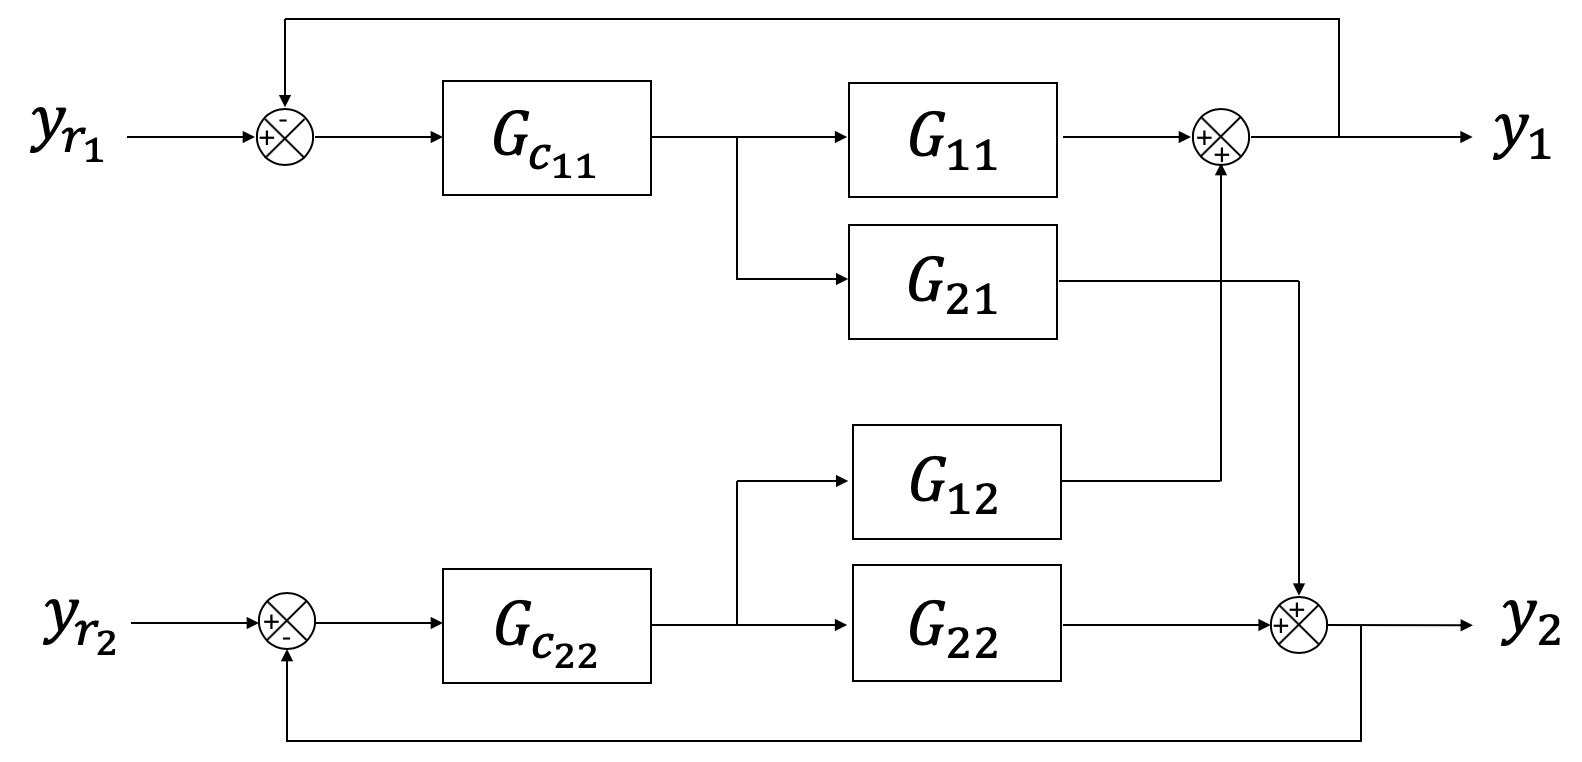
\includegraphics[scale=0.45]{images/pid_loop_iol.png}
    \caption{Simplified control system of the Wood-Berry distillation tower.}
    \label{fig: control_loop_IOL}
\end{figure}

\begin{equation}
    \centering
    G_{c}(s) = 
    \begin{bmatrix}
    g_{c_{11}}  &  0 \\ 
    0         &  g_{c_{22}}
    \end{bmatrix}
    \label{eq: controller_tf_iol}
\end{equation}

\begin{figure}[h]
    \centering
    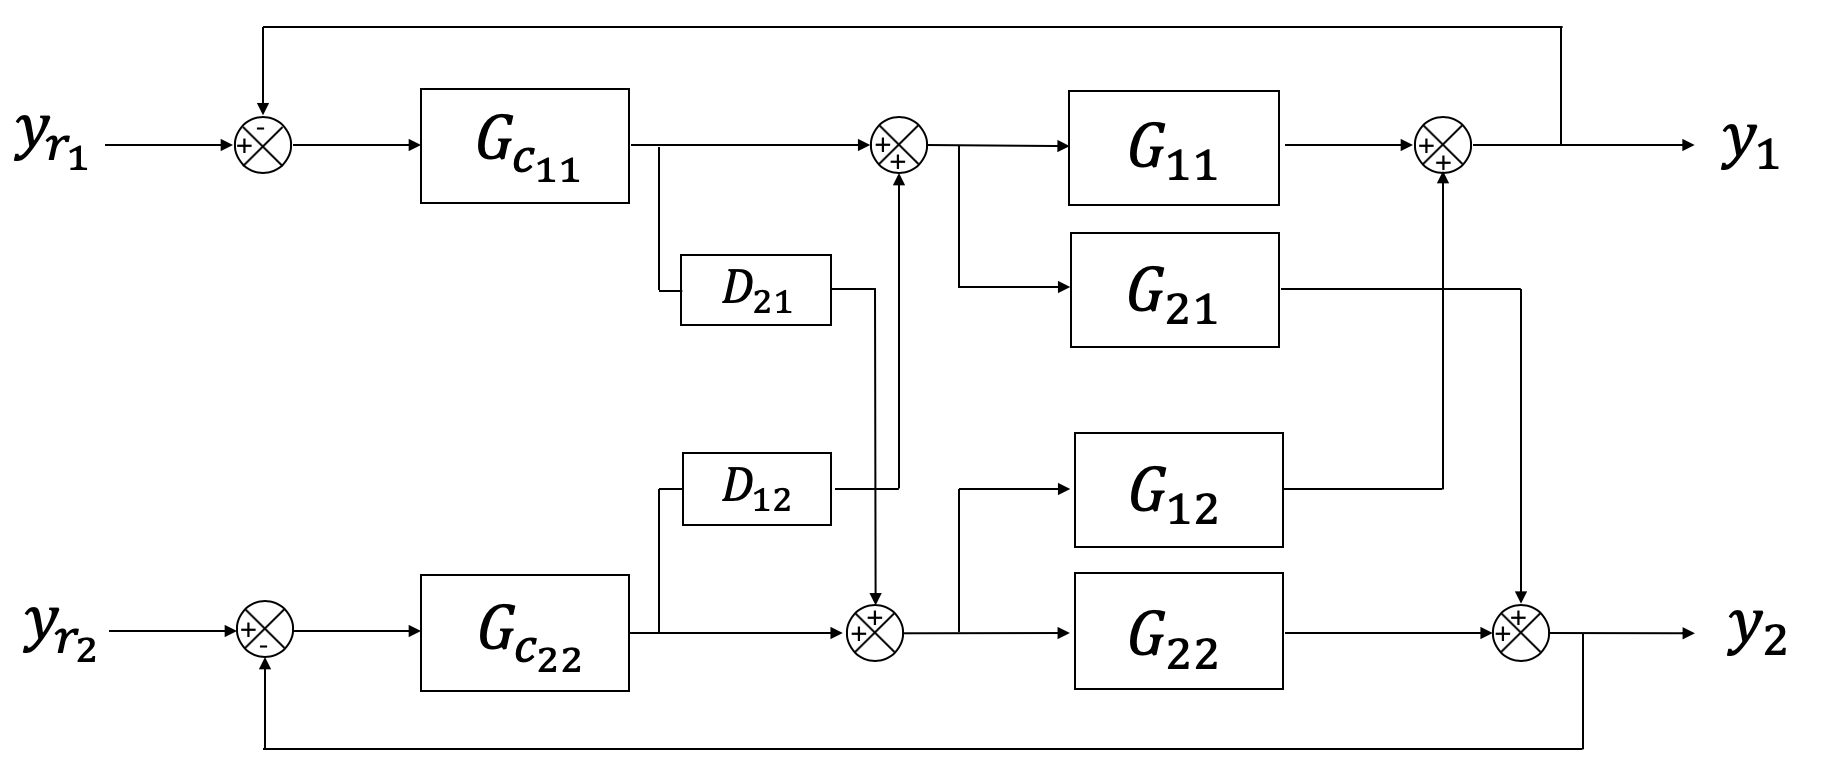
\includegraphics[scale=0.39]{images/decoupled_pid_loop_iol.png}
    \caption{Simplified decoupled control system of the Wood-Berry distillation tower.}
    \label{fig: decoupled_control_loop_IOL}
\end{figure}

\section{Introduction to Fault Tolerant Control}

Inevitably, all process equipment such as sensors, actuators, pumps, will malfunction or breakdown along their operational lifetime. Therefore, it is desirable to to have a fault tolerant control system (FTCS) in place to accommodate for these inevitable failures and ensure an acceptable level of performance during such events. The application of FTCS in the industrial environment results in increased operation robustness, production, and safety. The complete fault tolerant control system requires two algorithms: i) Fault prediction system to identify the location and type of fault. ii) Fault tolerant controller to "safe land" the process during a fault positive situation \cite{process_faults}.  This particular study is only concerned with the fault tolerant controller design, and assumes that the fault is appropriately identified using existing methods.

One area identified for potential reinforcement learning application is in the design of a fault tolerant controller.  Fault tolerant controllers activate when a process fault occurs, rendering normal controllers useless [citation required]. The objective of fault tolerant controllers are to guide the process out of the fault situation safely.  Subsequently, process engineers can diagnose the problem and re-activate the normal process controllers when deemed acceptable.  

Farivar and Ahmadabadi (2015) has designed fault tolerant controllers using reinforcement learning for a class of unknown linear systems \cite{ahmad}.  Zhang and Gao (2018) applied reinforcement learning fault tolerant controllers to flux cored wired systems \cite{zhang_gao}.  In this project, a reinforcement learning fault tolerant controller will be built for the mitigation of flooding in an industrial distillation tower. 

\section{Controlling using PID}
A PI controller was selected instead of a P or PID controller, because PI controllers are shown to achieve superior control performances compared to their counterparts \cite{PI_controller}.

\section{Controlling using MPC}
\section{Controlling using Reinforcement Learning}
\section{Comparison of Performance}